\documentclass[border=10pt]{standalone}
\usepackage{tikz}
\usetikzlibrary{arrows.meta,positioning,calc,decorations.pathmorphing}
\usepackage{amsmath,amssymb}

\begin{document}
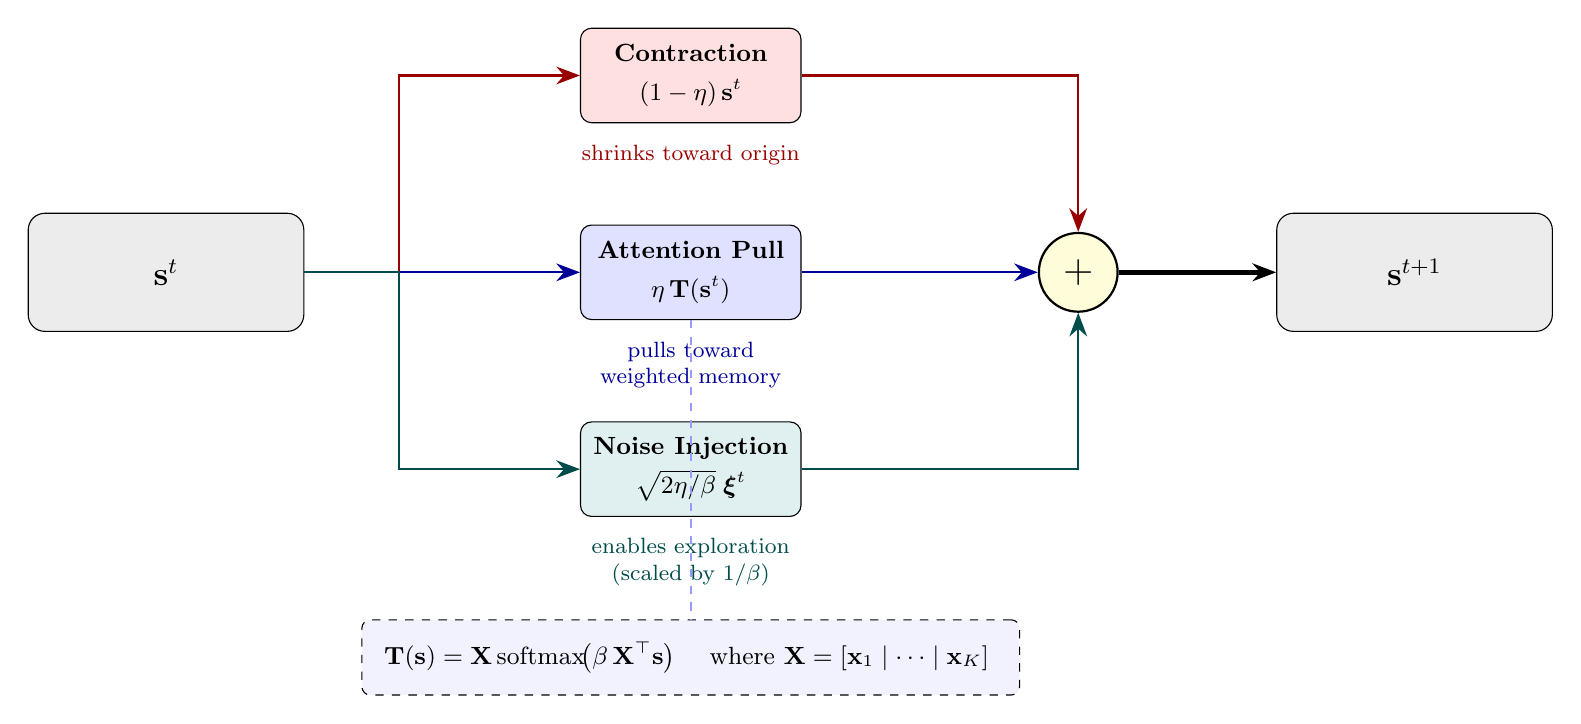
\begin{tikzpicture}[
    block/.style={rectangle, draw, rounded corners=4pt, minimum width=2.8cm, minimum height=1.2cm, align=center, font=\small},
    bigblock/.style={rectangle, draw, rounded corners=6pt, minimum width=3.5cm, minimum height=1.5cm, align=center, font=\normalsize},
    arr/.style={-{Stealth[length=3mm]}, thick},
    node distance=1.8cm and 2.5cm,
]

% Current state
\node[bigblock, fill=gray!15, font=\large] (st) {$\mathbf{s}^t$};

% Three terms
\node[block, fill=red!12, right=3.5cm of st, yshift=2.5cm] (contract) {
    \textbf{Contraction}\\[3pt]
    $(1-\eta)\,\mathbf{s}^t$
};

\node[block, fill=blue!12, right=3.5cm of st, yshift=0cm] (attention) {
    \textbf{Attention Pull}\\[3pt]
    $\eta\,\mathbf{T}(\mathbf{s}^t)$
};

\node[block, fill=teal!12, right=3.5cm of st, yshift=-2.5cm] (noise) {
    \textbf{Noise Injection}\\[3pt]
    $\sqrt{2\eta/\beta}\;\boldsymbol{\xi}^t$
};

% Sum node
\node[circle, draw, thick, fill=yellow!15, minimum size=1cm, font=\Large,
      right=3cm of attention] (sum) {$+$};

% Next state
\node[bigblock, fill=gray!15, font=\large, right=2cm of sum] (st1) {$\mathbf{s}^{t+1}$};

% Arrows from s^t to three terms
\draw[arr, red!60!black] (st.east) -- ++(1.2,0) |- (contract.west);
\draw[arr, blue!60!black] (st.east) -- (attention.west);
\draw[arr, teal!60!black] (st.east) -- ++(1.2,0) |- (noise.west);

% Arrows from three terms to sum
\draw[arr, red!60!black] (contract.east) -| (sum.north);
\draw[arr, blue!60!black] (attention.east) -- (sum.west);
\draw[arr, teal!60!black] (noise.east) -| (sum.south);

% Arrow from sum to next state
\draw[arr, black, ultra thick] (sum.east) -- (st1.west);

% Annotations below
\node[font=\footnotesize, red!60!black, below=0.15cm of contract, align=center] {shrinks toward origin};
\node[font=\footnotesize, blue!60!black, below=0.15cm of attention, align=center] {pulls toward\\weighted memory};
\node[font=\footnotesize, teal!60!black, below=0.15cm of noise, align=center] {enables exploration\\(scaled by $1/\beta$)};

% Attention detail box
\node[draw, dashed, rounded corners=3pt, fill=blue!5, font=\small,
      below=3.8cm of attention, minimum width=6cm, align=center, inner sep=8pt] (detail) {
    $\mathbf{T}(\mathbf{s}) = \mathbf{X}\,\mathrm{softmax}\!\bigl(\beta\,\mathbf{X}^\top\mathbf{s}\bigr)$
    \quad where $\mathbf{X} = [\mathbf{x}_1 \mid \cdots \mid \mathbf{x}_K]$
};

\draw[dashed, blue!40, thick] (attention.south) -- (detail.north);

\end{tikzpicture}
\end{document}
